\documentclass[a4paper,10pt]{article}

\usepackage{subfig}
\usepackage{float}
\usepackage{graphicx}

%opening
\title{A Social Network Model}
\author{Sam Magura, Vitchyr Pong}

\begin{document}

\maketitle

\section{Introduction}

In this social network model, we choose a node and break one of its incident edges. The model is speical in that the node is less likely to break a connection with a high-degree neighbor. This behavior reflects real social behavior; relationships with popular, well-connected people are potentially more valuble than relationships with less well-connected people. The model takes a parameter $I$ --- a measure of \emph{intolerance} toward unpopular people --- that determines the extent to which the degrees of adjacent nodes affect the breaking probabilities. We predicted that changing $I$ would make the model behave differently, but our simulations showed no relationship between $I$ and the model's macroscopic behavior. 

\section{Model Definition}

The process operates on a graph $G = (V, E)$. An iteration consists of the following steps. 

\begin{enumerate}
 \item Chose a vertex $v_0$ randomly from the set of all vertices with degree 1 or greater. 
 \item Exactly one edge incident to $v_0$ will be broken. For an edge $e^*$ that is incident to $v_0$, let the chance that $e^*$ is broken be proportional to

 \begin{equation}
\label{eqn:pr-function}
  \frac{I}{deg(v^*)} + \frac{1 - I}{deg(v_0)}
 \end{equation}

where $v^*$ is the \emph{other} vertex that $e^*$ is incident on. $I$ is in the range $[0, 1]$. Let this equation be known as the probability function. 

 \item Select a vertex $v'$ from $V \setminus \{v_0\}$. If there already exists an edge $(v_0, v')$, select a new $v'$ from $V \setminus \{v_0\}$. Continue to select vertices until a $v'$ that is not adjacent to $v_0$ is selected.

 \item Add an edge $(v_0, v')$ to the graph. 

\end{enumerate}

\section{Results}

We implemented the model in the Python programming language. In our implementation, the initial graph is $G(n, M)$ Erdos-Renyi random graph. We wrote an additional script to run the model many times with different values of $I$ to see if the behavior of the model depended on $I$ in a significant way. The script performed 1000 iterations for each trial. It then gathered several statistics on the resultant graph: number of nodes in largest component, diameter of largest component, and number of components. We predicted that the size and diameter of the largest component would increase with $I$, while the number of components would decrease with $I$. 

\begin{figure}[H]
\begin{center}
\subfloat{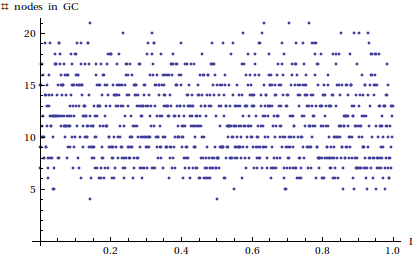
\includegraphics[height=4cm]{images/gc_size.png}}
\subfloat{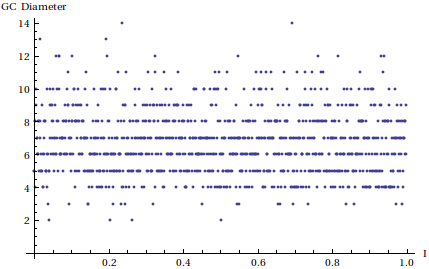
\includegraphics[height=4cm]{images/gc_diameter.png}}
\caption{Size and diameter of the largest component, for 40 nodes, 20 edges, and 1000 iterations per trial.}
\end{center}
\end{figure} 

\begin{figure}[H]
\begin{center}
\subfloat{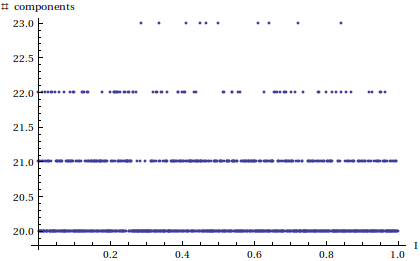
\includegraphics[height=4cm]{images/n_components.png}}
\subfloat{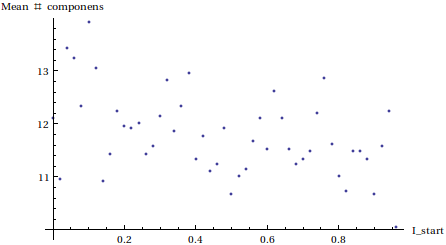
\includegraphics[height=4cm]{images/n_components_mean.png}}
\caption{Number of components and 20-trial means for number of components --- using 40 nodes, 20 edges, and 1000 iterations per trial.}
\end{center}
\end{figure} 

We did not notice a substantial correlation between $I$ and the size of largest component, the diameter of the largest component, or the number of components. There appears to be a very slight negative correlation between $I$ and the 20-trial number-of-component means.

In order to see why there were no correlations, we tracked the size and diameter of the largest component of the graph as iterations were performed. The following plot of size of largest component versus iteration number $i$ explains why there were no correlations. 

\begin{figure}[H]
\label{fig:gc-size-iter}
\begin{center}
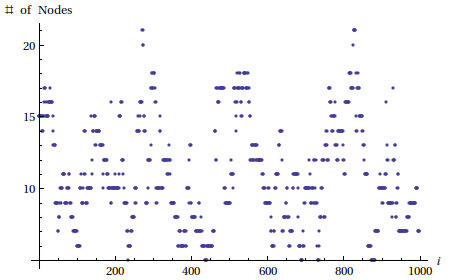
\includegraphics[height=5cm]{images/gc_size_iter.png}
\caption{How the size of the largest component changes as iterations are performed. The plot for diameter of largest component was similar.}
\end{center}
\end{figure} 
The plot shows that the model is not stable, i.e. the size of the largest component does not approach a specific value. This is to be expected because an edge is broken each iteration, no matter what. The previous plot shows that, often times, over half of the graph's 20 edges are in the largest component. In an iteration where one of these edges is broken, the size of the largest component can only decrease or remain the same. Additionally, the value of $I$ does not restrict the graph from reaching any given state; at most, the value of $I$ could make a certain state less likely to reach. With the size of the largest component ranging from 5 to 21 --- for a graph with 40 nodes and 20 edges --- the existence of a correlation between this property of the graph and $I$ seems unlikely.

\subsection{Model Variations}
In attempt to get more interesting results, we tried several changes to the model. None of the changes produced correlations between $I$ and any of the three quantities we recorded.

\begin{itemize}

 \item We tried to change the probability function to increase the effect of $I$ on the breaking probabilities. For example,
 \begin{equation}
  \frac{I^2}{deg(v^*)} + \frac{(1 - I)^2}{deg(v_0)}
 \end{equation}
and
 \begin{equation}
  \frac{sin(\frac{\pi}{4}I)}{deg(v^*)} + \frac{cos(\frac{\pi}{4}I)}{deg(v_0)}.
 \end{equation}

 \item Instead of using a probability function, we modified the model so that $v_0$ would always break its connection with its neighbor of least degree --- and if there were multiple neighbors of least degree, chose which one to break with randomly. 

\end{itemize}
 None of these changes produced correlations.

\end{document}
